\chapter{TABLES, FIGURES AND MATRICES}
\label{chap-two}
In Chapter \ref{chap-one} we did some typesetting and equations; now let's 
look at tables, figures, and matrices.

\section{Tables}
Table \ref{tab:one} is about as simple as they come, to put a formula in a 
table just use the same methods as putting a formula in a paragraph.  
Table \ref{tab:two} is a similar table in landscape on a seperate page.  
%
\begin{table}
\caption{Table Example}
\label{tab:one}
\begin{center}
\begin{tabular}{lccl}
\toprule
Treatment & No Death & Death & Total\\
\midrule
Therapy A & 1295 & 72 & 1367\\
Therapy B 	& 2294 & 195 & 2489\\
\midrule
Total & 3589 & 267 & 3856\\
\bottomrule
\end{tabular}
\end{center}
\end{table}

\paragraph{Filler Text} \lipsum[1-2]
\newgeometry{margin=1in,lmargin=1.25in,footskip=\chapterfootskip, includehead, includefoot}
%\thispagestyle{lscape}
%\pagestyle{lscape}
\thispagestyle{lscapedplain}
\begin{landscape}
\begin{table}
\caption{Landscape Table Example}
\label{tab:two}
\begin{center}
\begin{tabular}{lcccccccccl}
\toprule
Patient & A & B & C & D & E & F & G & H &I & Total \\
\midrule
John & 1 & 2 & 3 & 4 & 5 & 6 & 7 & 8 & 9 & 45 \\
Amy & 1 & 2 & 3 & 4 & 5 & 6 & 7 & 8 & 9 & 45 \\
Jim & 1 & 2 & 3 & 4 & 5 & 6 & 7 & 8 & 9 & 45 \\
Jason & 1 & 2 & 3 & 4 & 5 & 6 & 7 & 8 & 9 & 45 \\
Sandy & 1 & 2 & 3 & 4 & 5 & 6 & 7 & 8 & 9 & 45 \\
Icem & 1 & 2 & 3 & 4 & 5 & 6 & 7 & 8 & 9 & 45 \\
\midrule
Total & 6 & 12 & 18 & 24 & 30 & 36 & 42 & 48 & 54 & 270\\
\bottomrule
\end{tabular}
\end{center}
\end{table}
\end{landscape}
%\newgeometry{margin=1in,lmargin=1.25in,footskip=\chapterfootskip, includehead, includefoot,landscape=false}
\restoregeometry
\pagestyle{plain}
\thispagestyle{plain}
\newgeometry{margin=1in,lmargin=1.25in,footskip=\chapterfootskip, includehead, includefoot}


\section{Figures}

The easiest way to insert a picture is to have that picture in pdf format.  
\fref{fig:hist1} and \fref{fig:hist2} are two figures typeset normally.
ETD guidelines allow the use of landscape pages in the electronic 
submission.  To rotate a page, do NOT use the \texttt{lscape} environment. Instead, use the \texttt{pdflscape} package, for compatibility with PDFlatex.
Please note, if you are preparing a document for binding, consider
giving the \texttt{hardcopy} option in the \verb|\documentclass|
declaration.  This will place the page number at the normal location,
which is where it should be for printing and binding.
%
\begin{figure}[hbtp]
\centering
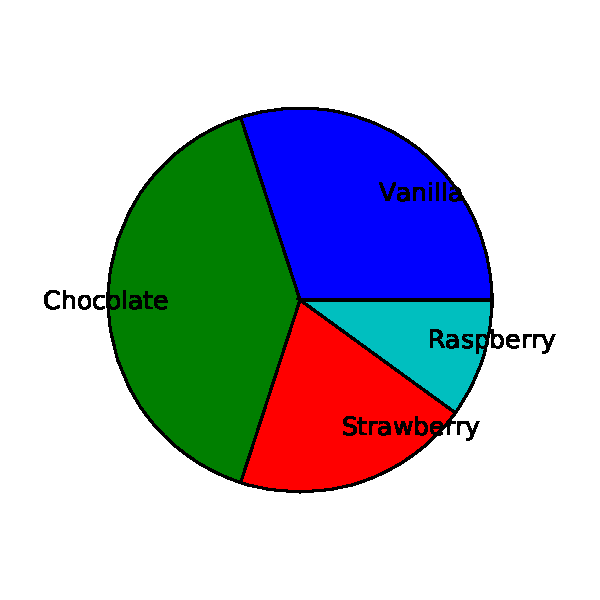
\includegraphics[width=0.6\textwidth]{Chapter-2/figs/pie}
\caption{Here is a sample figure}
\label{fig:hist1}
\end{figure}

For an example of a figure with a really long caption, see Fig.~\ref{fig:longcap}
\begin{figure}[hbtp]
\centering
\calculategraphicstargetheight{11}
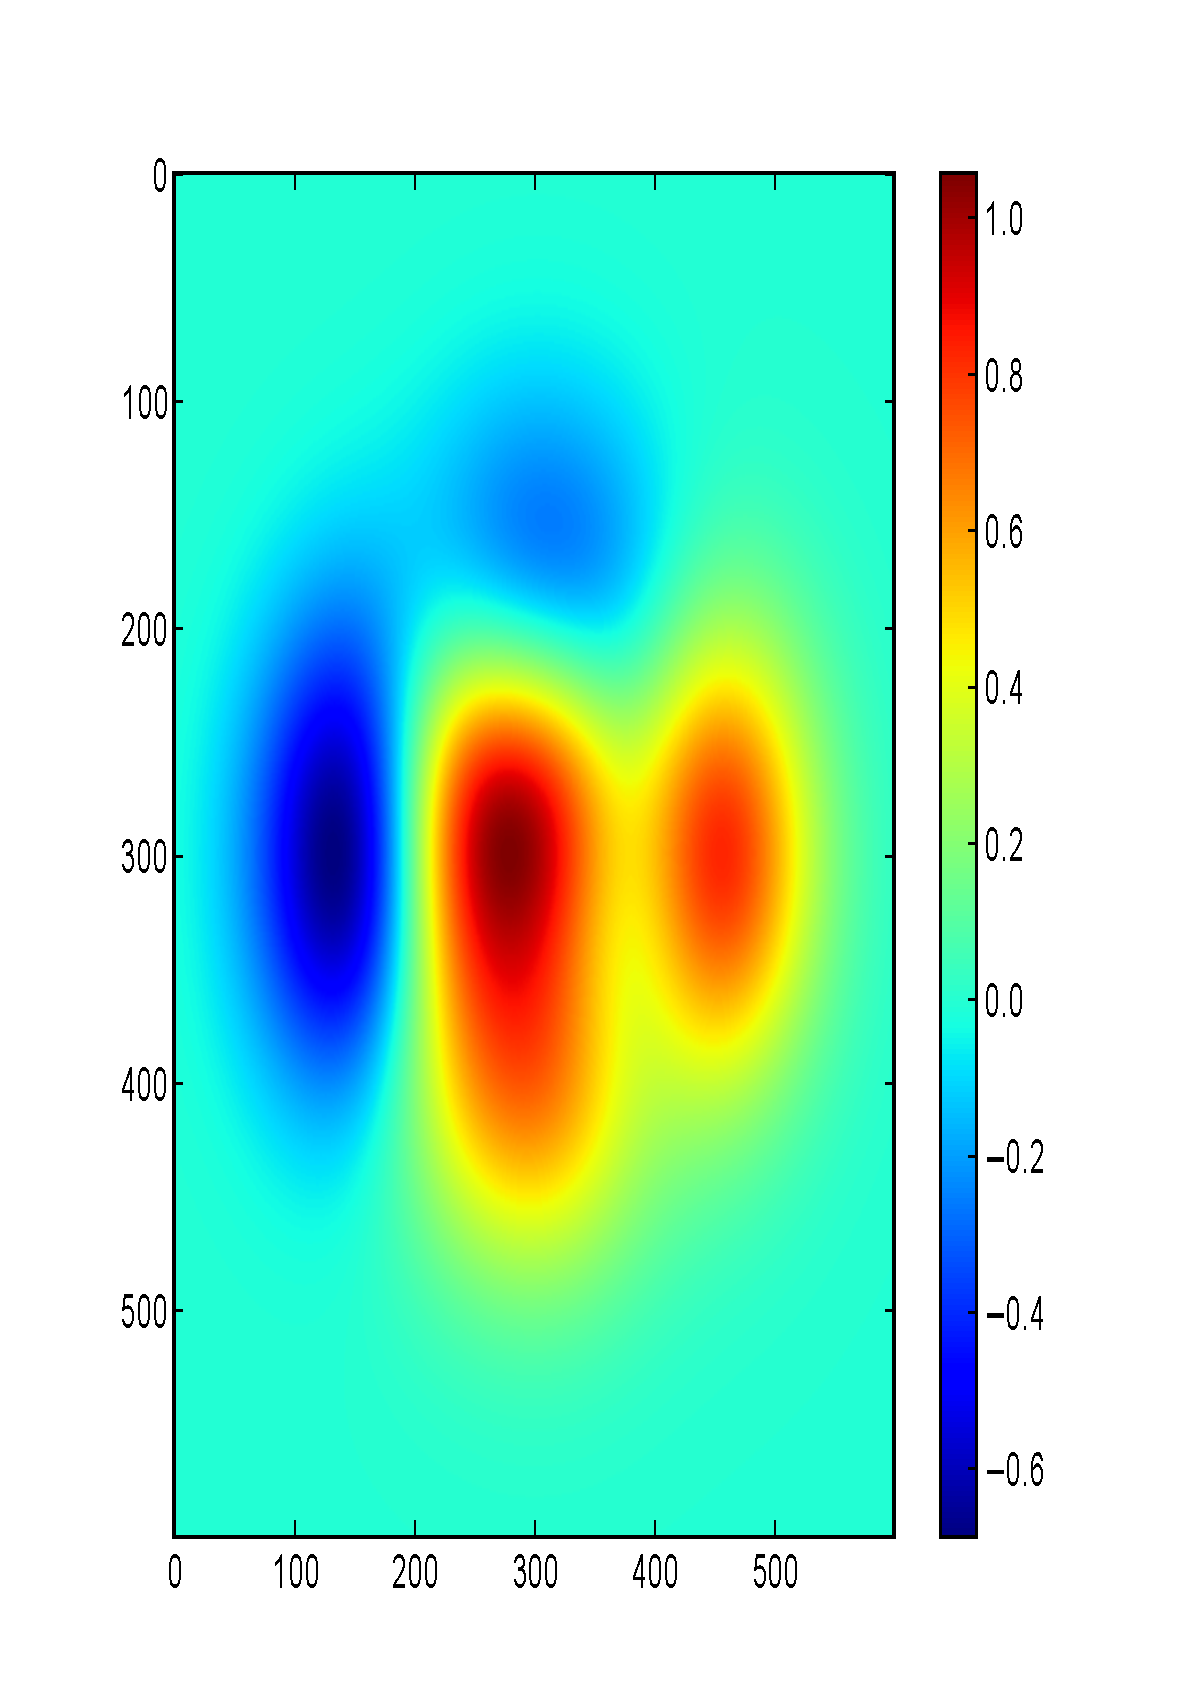
\includegraphics[height=\graphht]{Chapter-2/figs/color_stretched}
\caption{Here is a HUGE sample figure with a HUGE caption. Our goal is to make a caption that is so long that the caption spills into the lower margin, leading to an ETD error. The way to solve this problem in a systematic way is to calculate how many lines of text the caption will use, then adjust the size of the image, such that it leaves just enough space for your huge caption. How I am solving this problem is by providing a new variable called graphht that stores how tall the image should be. Then, to calculate how tall to make the figure, you use the new function that I am providing called calculategraphicstargetheight. This function has one argument. The argument of the function is how many lines of text you estimate that the caption occupies. You can always run your tex once, measure this number, and type it into the argument for the function. What the function will do (it is defined in the preamble) is take into account the size you give it, the spacing of the chapter and the footer at the bottom, 
and then calculate the total vertical space available. Thus, this function should be used for images that are taller than they are wide.}
\label{fig:longcap}
\end{figure}
%
\begin{figure}[hbtp]
\centering
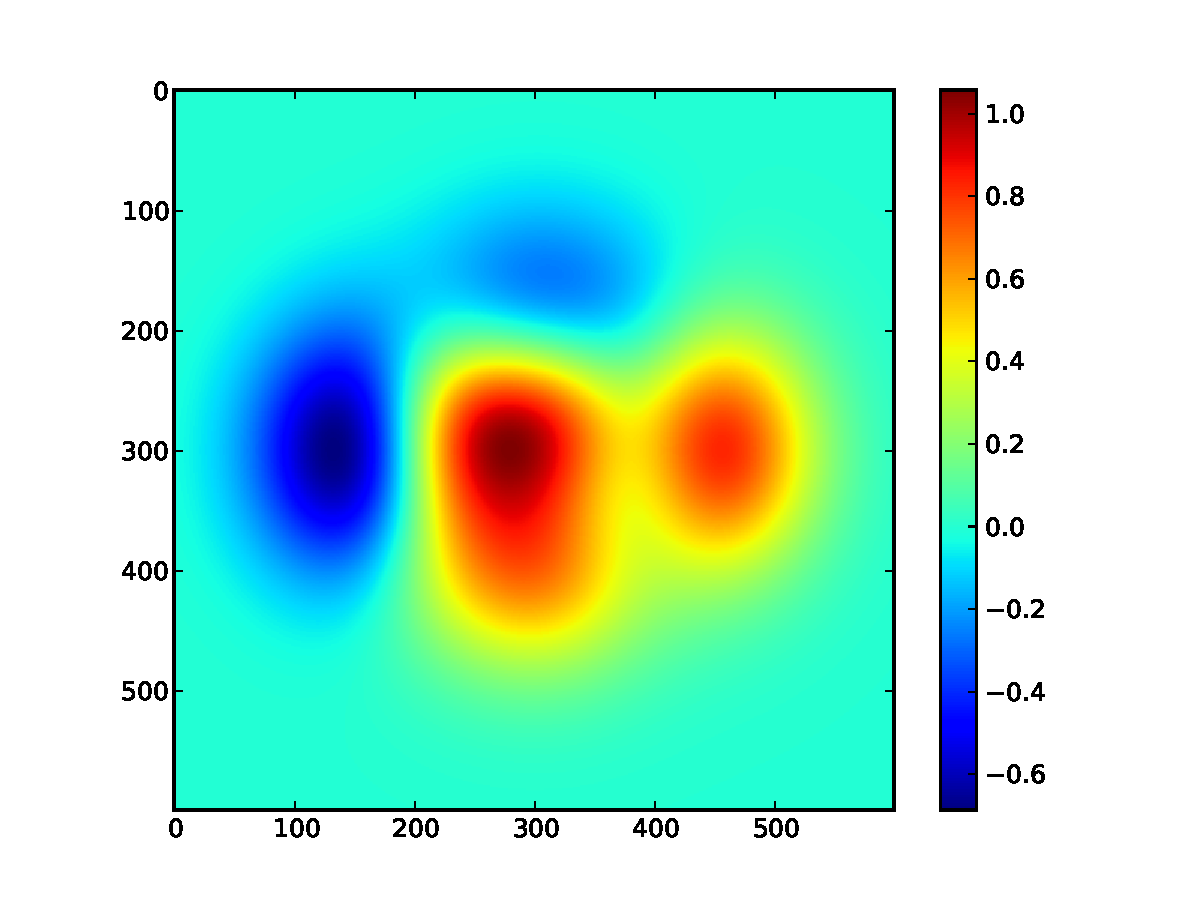
\includegraphics[width=0.6\textwidth]{Chapter-2/figs/color}
\caption{Here is a sample figure}
\label{fig:hist2}
\end{figure}
%
\begin{figure}[hbtp]
\centering
\subfloat[]{
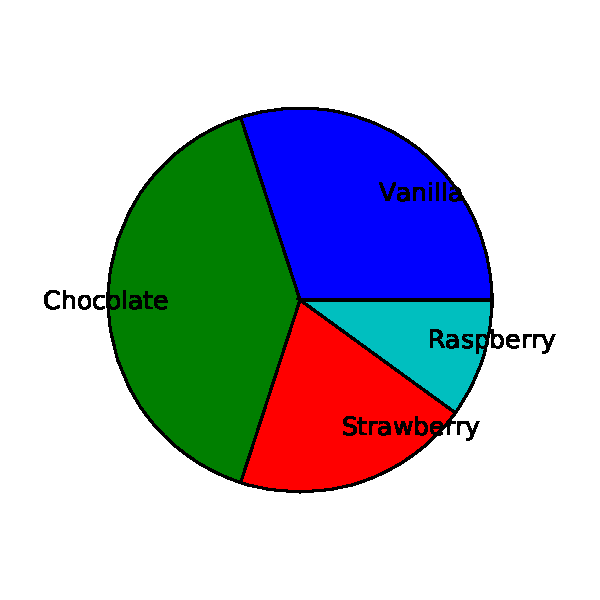
\includegraphics[width=0.4\textwidth]{Chapter-2/figs/pie}
}
\subfloat[]{
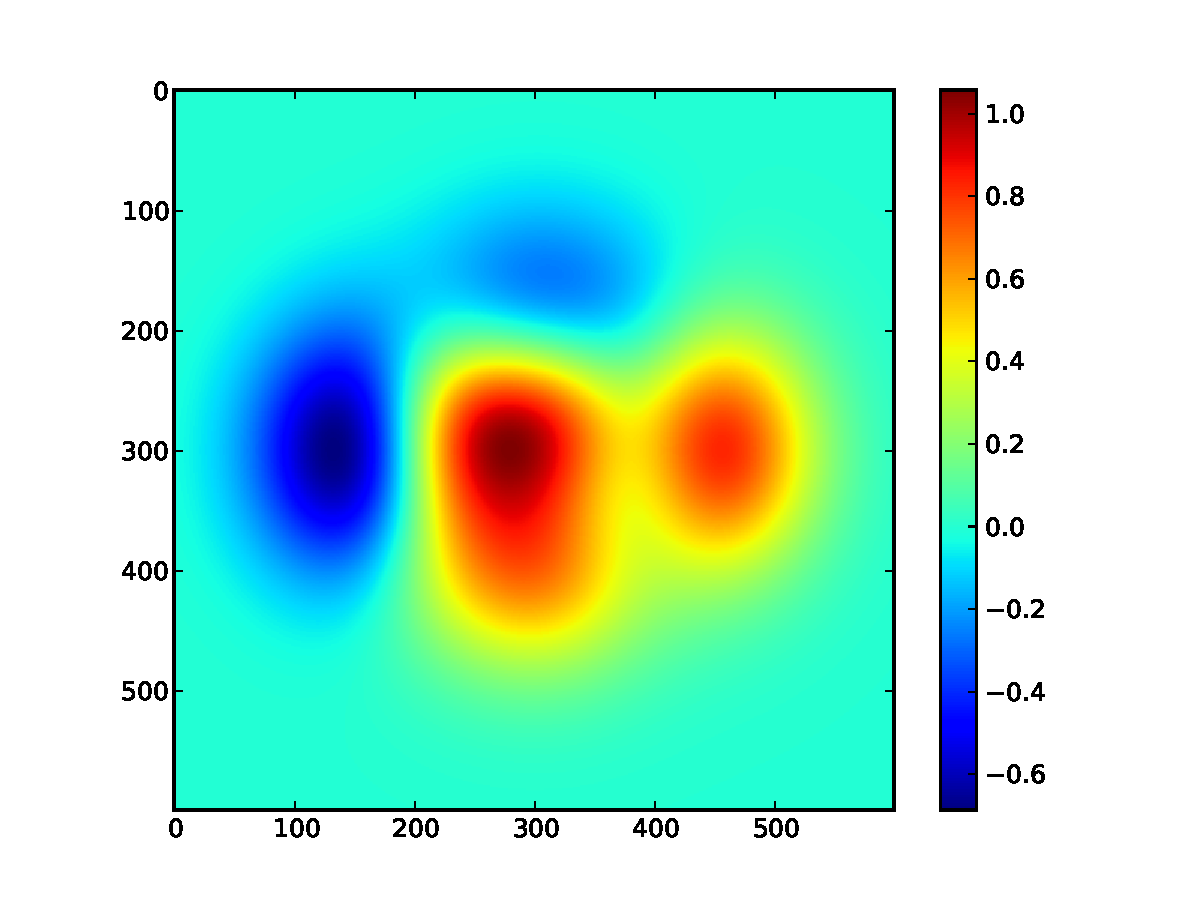
\includegraphics[width=0.4\textwidth]{Chapter-2/figs/color}
}
\caption{Here are two floating subfigures}
\label{fig:subfigures}
\end{figure}


\paragraph{Filler Text} \lipsum[12-15]

\newgeometry{margin=1in,lmargin=1.25in,footskip=\chapterfootskip, includehead, includefoot}
%\thispagestyle{lscaped}
%\pagestyle{lscaped}
\thispagestyle{lscapedplain}
\begin{landscape}
\begin{figure}
\centering
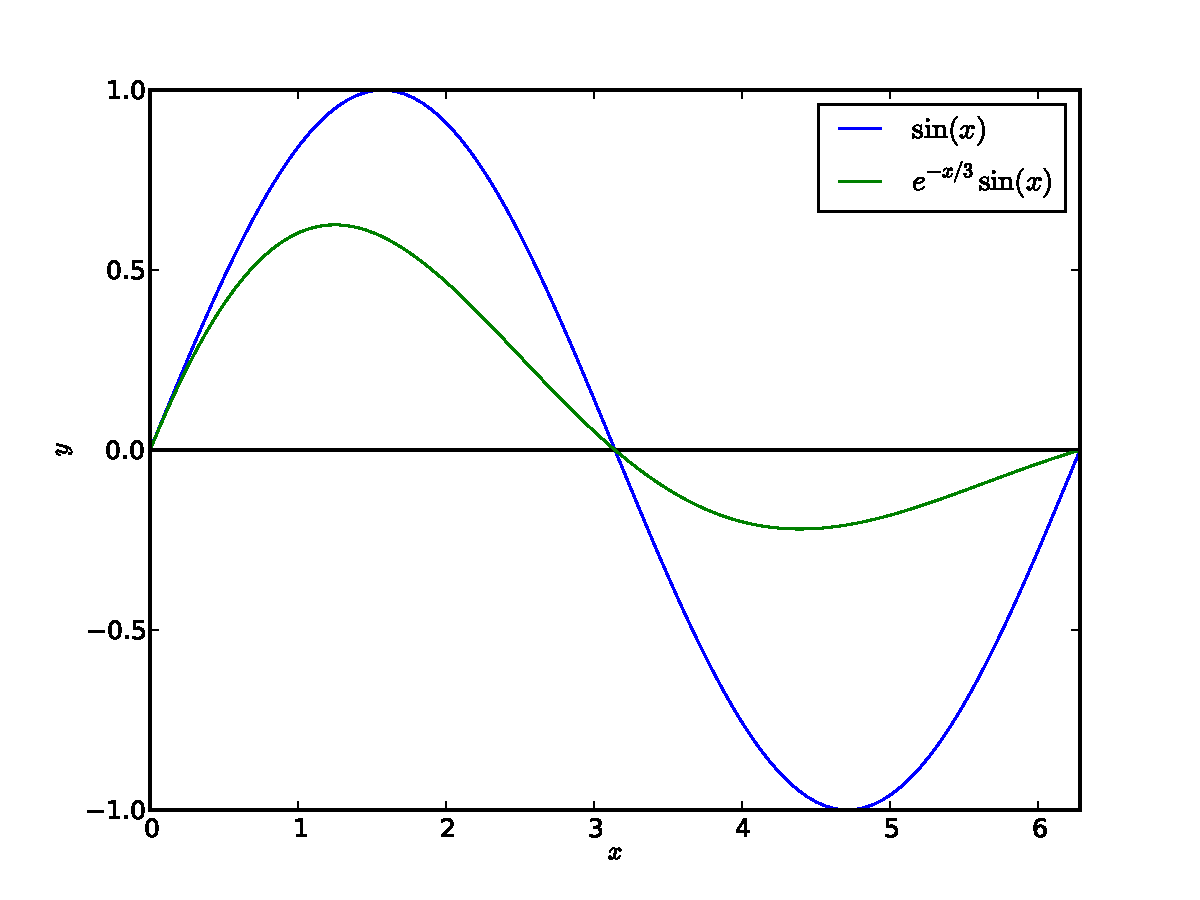
\includegraphics[width=\textwidth]{Chapter-2/figs/sine}
%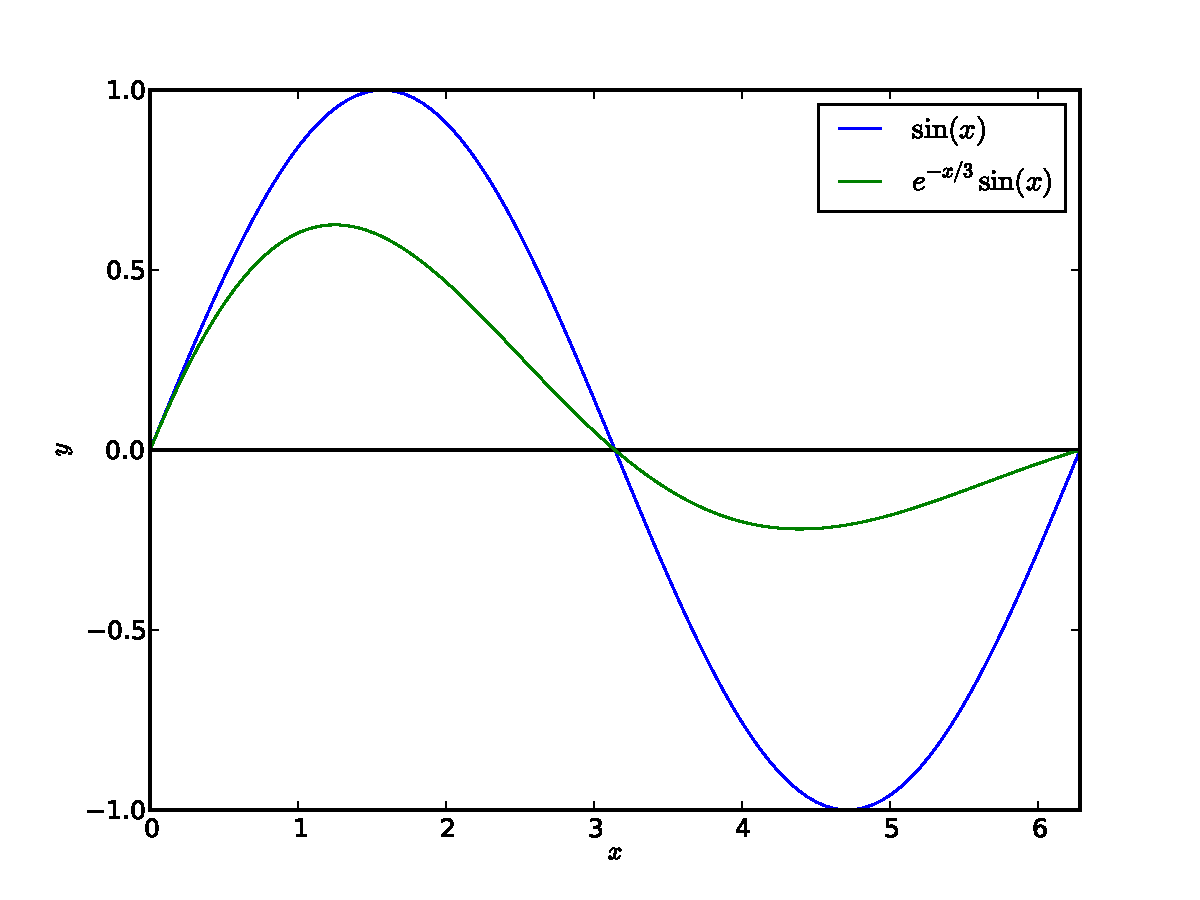
\includegraphics[height=\textwidth]{Chapter-2/figs/sine}
\caption{This figure has been turned sideways.  With large figures, 
         the author must ensure that there are at least two double spaces
         between the caption and the page number.}
\label{fig:hist}
\end{figure}
\end{landscape}
%\newgeometry{margin=1in,lmargin=1.25in,footskip=\chapterfootskip, includehead, includefoot,landscape=false}
\restoregeometry
\pagestyle{plain}
\thispagestyle{plain}
\newgeometry{margin=1in,lmargin=1.25in,footskip=\chapterfootskip, includehead, includefoot}


\section{Matrices}
Let's look at a simple example of a matrix:
\[ \left( \begin{array}{ccc}
a & b & c \\
d & e & f \\
g & h & i \end{array} \right)\] 
%
You may prefer to write it this way:
\[ \left[\begin{array} {cccccc}
1 & 0 & 0 & 0 & 0 & 0 \\
0 & 1 & 0 & 0 & 0 & 0 \\
0 & 0 & 1 & 0 & 0 & 0 \\
0 & 0 & 0 & 1 & 0 & 0 \\
0 & 0 & 0 & 0 & 1 & 0 \\
0 & 0 & 0 & 0 & 0 & 1 \\
\end{array} \right] \]
